\documentclass[10pt,a4paper]{article}
\usepackage[utf8]{inputenc}
\usepackage[T1]{fontenc}
\usepackage[french]{babel}
\usepackage{fourier} %Nécessaire pour faire des jolis attention
\usepackage{supertabular} %Nécessaire pour les longs tableaux
\usepackage[top=2.2cm, bottom=2.5cm, right=2.5cm, left=2.5cm]{geometry} %Mise en page
\usepackage{amsmath} %Nécessaire pour les maths
\usepackage{amssymb} %Nécessaire pour les maths
\usepackage{stmaryrd} %Utilisation des double crochets
%\usepackage{pifont} %Utilisation des chiffres entourés
\usepackage{graphicx} %Introduction d images
\usepackage{epstopdf} %Utilisation des images .eps
\usepackage{amsthm} %Nécessaire pour créer des théorèmes
\usepackage{algorithmic} %Nécessaire pour écrire des algorithmes
\usepackage{algorithm} %Idem
\usepackage{bbold} %Nécessaire pour pouvoir écrire des indicatrices
\usepackage{hyperref} %Nécessaire pour écrire des liens externes
\usepackage{array} %Nécessaire pour faire des tableaux
\usepackage{tabularx} %Nécessaire pour faire de longs tableaux
\usepackage{caption} %Nécesaire pour mettre des titres aux tableaux (tabular)
\usepackage{color} %nécessaire pour écrire en couleur
\usepackage{float} % Pour l'option [H] de \begin{figure}
\newtheorem{thm}{Théorème}
\newtheorem{mydef}{Définition}
\newtheorem{prop}{Proposition}
\newtheorem{lemma}{Lemme}

\newcommand{\hmm}{\textsc{HMM}}
\newcommand{\mcmc}{\textsc{MCMC}}
\newcommand{\fhmm}{\textsc{Factorial HMM}}
\newcommand{\Estep}{\textsc{E-step}}
\newcommand{\Mstep}{\textsc{M-step}}
\newcommand{\EM}{\textsc{EM}}

\title{MVA, Projet optimisation : Inégalité linéaires}
  \author{Valentin \textsc{De Bortoli}, Louis \textsc{Thiry}}
\begin{document}
\maketitle
\tableofcontents

\section{Présentation du problème}

On s'intéresse aux problèmes d'égalité et d'inégalité aux moindres carrés.

\begin{mydef}
  Soient $A \in \mathcal{M}_{n,m}(\mathbb{R})$ avec $(n,m) \in \mathbb{N}^2$ et $b \in \mathbb{R}^{n}$.
    On appelle problème d'égalité aux moindres carrés et on note $\mathcal{P}_{=} (A, b)$ le probleme de minimisation :
    \begin{align*}
      \mathcal{P}_{=}(A, b): \quad & \hat{x} = \underset{x}{\text{argmin }}  ||Ax - b||^{2}\\
    \end{align*}
\end{mydef}
Résoudre le problème d'égalité aux moindres carrés permet de trouver la meilleure solution possible au systeme linéaire $Ax = b$ :
\begin{itemize}
  \item lorsqu'il existe une solution à ce système linéaire, les deux problèmes sont équivalents
  \item si $b$ n'est pas dans l'images de $A$ , où bien lorsque l'on a plus d'équations que d'inconnues $(n > m)$ et est inconsistant, il n'y a aucune solutions.
    Dans ce cas, une solution $x_0$ du problème d'égalité aux moindres carrés est la meilleure approximations telle que $Ax_0 = b$ au sens des moindres carrés.
    C'est une solution approximative au système linéaire $Ax = b$
\end{itemize}

\begin{mydef}
  On appelle problème d'inégalité aux moindres carrés et on note $\mathcal{P}_{\leq} (A, b)$ le probleme de minimisation :
    \begin{align*}
      \mathcal{P}_{\leq} (A, b): \quad & \hat{x} = \underset{x}{\text{argmin }}  ||(Ax - b)_+||^{2}\\
    \end{align*}
\end{mydef}
De même que pour le cas d'égalité, résoudre le problème d'inégalité aux moindres carrés permet de trouver la meilleure solution possible au systeme d'inégalité linéaires $Ax \leq b$ :
\begin{itemize}
  \item lorsqu'il existe une solution à ce système d'inégalité, les deux problèmes sont équivalents
  \item Dans le cas où ils n'y a pas de solutions aux système d'inégalité, c'est une solution approximative.
\end{itemize}

Le problème d'égalité est bien compris: on connait la forme des solutions.
Ce problème est traité dans la première partie du rapport.

Pour le problème d'inégalité, on a simplement un résultat d'existence.

\textbf{Le but de ce rapport est de proposer un algorithme pour trouver une solution au problème d'intégalité aux moindres carrés $\mathcal{P}_{\leq} (A, b)$.}

\section{Egalité aux moindres carrés}

\subsection{Rappels sur la pseudo-inverse}

On introduit la notion de matrice pseudo inverse de Moore-Penrose \cite{penrose1955generalized} qui joue un rôle particulier dans l'étude des problèmes aux moindres carrés.
\begin{thm}
Soit $A \in \mathcal{M}_{n,m}(\mathbb{R})$ avec $(n,m) \in \mathbb{N}^2$.
Il existe $(M,N)$ deux matrices orthogonales de $\mathcal{M}_m(\mathbb{R)}$, respectivement $\mathcal{M}_n(\mathbb{R})$ et $\Sigma=\left( \begin{matrix}
D & 0 \\ 0 & 0
\end{matrix}\right)$ avec $D$ diagonale strictement positive telles que $A=N\Sigma M$.
\end{thm}
\subparagraph{Démonstration :} On considère la matrice $A^TA \in \mathcal{M}_{m}(\mathbb{R})$.
Celle-ci est symétrique, semi-définie positive et on peut appliquer le théorème spectral.
On a donc une matrice orthogonales $P$ qui vérifient $P^TA^TAP=\begin{matrix}
D^2 & 0 \\ 0 & 0
\end{matrix}$ avec $D^2$ diagonale strictement positive.
Il est à noter que $D$ est une matrice de $\mathcal{M}_r(\mathbb{R})$ où $r$ est le rang de la matrice $A$ (et donc plus petit que $m$ et $n$).
On note $P=[P_1 \ P_2]$ où $P_1 \in \mathcal{M}_{m,r}(\mathbb{R})$ et $P_2 \in \mathcal{M}_{m,m-r}(\mathbb{R})$.
On a alors :
\begin{equation}
\left\lbrace
\begin{aligned}
P_1^T A^T A P_1 = D^2 \\
P_1^T A^T A P_2 =0 \\
P_2^T A^T A P_1 =0 \\
P_2^T A^T A P_2 =0
\end{aligned}
\right.
\end{equation}
Posons $Q_1=A P_1 D^{-1}$.
On a bien
  $Q_1^T Q_1 = D^{-1} P_1^T A^T A P_1 D^{-1} = Id_r$.
On complète $Q_1$ en une matrice orthogonale de $\mathcal{M}_n(\mathbb{R})$ et on a
  $Q^T A P=
  \left( \begin{matrix}
    D P_1^T A^T A P_1 & D P_1^T A^T A P_2 \\
    Q_2^T A P_1 & Q_2^T A^T A P_2
  \end{matrix} \right)$.
Or
  $P_1^T A^T A P_2=0$
et
  $Q_2^T Q_1=D Q_2^T A P_1 =0$
et puisque
  $P_2^T A^T A P_2=0$
, $A P_2=0$.
Donc on trouve bien
  $Q^T A P =
    \left( \begin{matrix}
      D & 0 \\
      0 & 0
    \end{matrix}\right)$.\\
On peut alors définir la pseudo-inverse.
\begin{mydef}[Pseudo-inverse de Moore-Penrose, 1920]
On appelle pseudo-inverse de Moore-Penrose de $A$ et on note $A^+$ la matrice $A^+=M^T \left( \begin{matrix}
D^{-1} & 0 \\ 0 & 0
\end{matrix}\right)N^T \in \mathcal{M}_{m,n}(\mathbb{R})$ (où $M, N$ sont les matrices orthogonales qui apparaissent dans la décomposition en valeurs singulières).
\end{mydef}
\begin{prop}
$A^+$ vérifie les propriétés suivantes :
\begin{itemize}
\item $A^+A A^+=A^+$
\item $A A^+ A =A$
\item $A A^+$ est symétrique
\item $A^+ A$ est symétrique
\end{itemize}
\end{prop}
On peut alors montrer la propriété suivante :
\begin{prop}
Il existe une unique matrice qui vérifie ces quatre propriétés, la pseudo-inverse de Moore-Penrose.
\end{prop}
\subparagraph{Démonstration :} Soient $(B,C)$ deux matrices satisfaisant les propriétés énoncées.
On a alors :
\begin{equation}
\begin{aligned}
AB&=ACAB \\
&=(AC)^T(AB)^T \\
&=(ABAC)^T \\
&=ABAC \\
&=AC
\end{aligned}
\end{equation}
De la même manière, $BA=CA$.
Ensuite on a :
\begin{equation}
\begin{aligned}
C&=CAC\\
&=CAB\\
&=BAB\\
&=B
\end{aligned}
\end{equation}
On établit maintenant une proposition concernant des décompositions orthogonales de l'espace.
\begin{prop}
On a les égalité suivantes :
\begin{itemize}
\item $\text{ker}A^T \overset{\perp}{\oplus} \text{Im}A = \mathbb{R}^m$
\item $\text{ker}A \overset{\perp}{\oplus} \text{Im}A^T = \mathbb{R}^n$
\item $\text{ker}A^+ \overset{\perp}{\oplus} \text{Im}A = \mathbb{R}^m$ et $AA^+$ projecteur orthogonal sur $\text{Im}A$ de noyau $\text{ker}A^+$
\item $\text{ker}A \overset{\perp}{\oplus} \text{Im}A^+ = \mathbb{R}^n$ et $A^+A$ projecteur orthogonal sur $\text{Im}A^+$ de noyau $\text{ker}A$
\end{itemize}
\end{prop}
\subparagraph{Démonstration :} concernant les deux premiers points, on vérifie rapidement l'orthogonalité de ces deux espaces.
Puis on peut conclure sur le fait que leur somme directe correspond bien à tout l'espace en utilisant un argument de dimension (notamment $\text{rg}A=\text{rg}A^T$).\\
Pour les deux autres points on ne démontre que le premier (le second s'effectue exactement de la même manière). $(AA^+)^2=AA^+$ donc c'est un projecteur et la condition de symétrie assure son orthogonalité. $\text{ker}A^+$ est trivialement inclus dans son noyau.
Soit un élément $x$ tel que $AA^+x=0$, alors $A^+AA^+x=A^+x=0$ donc c'est un élément du noyau de $A^+$.
On en déduit l'égalité des noyaux.
De plus $\text{Im}A \subset \text{Im}AA^+$.
Soit $y=Ax$.
Alors $y=AA^+Ax$ donc $y \in \text{Im}A$.
On a donc l'égalité des images.
On peut donc conclure.
\begin{prop}
Une conséquence de cette proposition est $\text{ker}A=\text{ker}A^+$ et $\text{Im}A=\text{Im}A^+$.
\end{prop}
\subparagraph{Remarque :} cette identification des supplémentaires est vraie seulement parce que les sommes directes sont orthogonales.\\

\subsection{Solutions au problème d'égalité aux moindres carrés}

Revenons au problème des moindres carrés.
\begin{prop}
  Un élément $x$ est solution du problème $\mathcal{P}_{=}(A, b)$ si et seulement si $A^T(Ax-b)=0$.
\end{prop}
\subparagraph{Démonstration :}
Le problème d'égalité aux moindre carrés consiste en la minimisation de la fonction $F: x \mapsto ||Ax - b||^2$.
F étant convexe, ses minimas sont ses points stationnaires, qui vérifient $\nabla F = 0$, i.e. $A^T(Ax - b) = 0$.

\begin{prop}
  L'ensemble des solutions du problème $\mathcal{P}_{=}(A, b)$ est l'ensemble $A^+b + \text{ker}A$.
\end{prop}
\subparagraph{Démonstration :}
  Une solution $x$ du problème vérifie $A^T(Ax-b)=0$ donc est solution du système linéraire $A^TAx = A^Tb$.
  L'ensemble des solutions de ce système linéaire est $x_0 + \text{ker}A^TA$ ou $x_0$ est une solution particulière ce ce système.
\begin{itemize}
  \item $A^+b$ est une solution particulière de ce système:
    \begin{align*}
      A^T A A^+ &= A^T (A A^+)^T \\
        &= (A A^+ A)^T\\
        &= A^T\\
      \implies &A^T A (A^+ b) = A^Tb\\
    \end{align*}
  \item $\text{ker}A = \text{ker}A^TA$.
    \begin{align*}
      \text{ker}A &\subset \text{ker}A^TA\\
      \text{ker}A^TA &\subset \text{ker}A:\quad x \in &\text{ker}A^TA \implies A^TAx = 0 \implies x^TA^TAx = 0 = || Ax ||^2 \implies Ax = 0 \implies x \in \text{ker}A\\
    \end{align*}
\end{itemize}
Donc l'ensemble des solutions du problème $\mathcal{P}_{=}(A, b)$ est $A^+b + \text{ker}A$.

\begin{prop}
  $A^+b$ est la solution de $\mathcal{P}_{=}(A, b)$ de norme minimale.
\end{prop}
\subparagraph{Démonstration :}
  Toute solutions $x_0$ de $\mathcal{P}_{=}(A, b)$ s'écrit $x_0 = A^+b + y$, $y \in \text{ker}A$.
  Comme $\text{ker}A \perp \text{Im}A^+$, par le théoreme de Pythagore $\|x_0 \|^2= \|A^+b \|^2 + \| y \|^2$ donc $\|x_0\| \leq \|A^+b\|$.

Maintenant que nous avons traité le problème d'égalité aux moindres carrés, intéressons nous au problème d'inégalité aux moindres carrés.

\section{Inégalité aux moindres carrés}

\subsection{Existence de solutions}

\begin{thm}
  Quelque soit la matrice $A \in \mathcal{M}_{n \times m}(\mathbb{R})$ et le vecteur $b \in \mathbb{R}^n$, le problème d'inégalité aux moindres carrés $\mathcal{P}_{\leq}(A, b)$ admet une solution $x_0 \in \mathbb{R}^m$.
  Quelque soit la solution $x_0$, le vecteur résidu $z = (Ax_0 - b)_+$ est unique est $x$ est une solution du problème ssi $(Ax - b)_+ = z$.
\end{thm}
\subparagraph{Démonstration :}
Pour l'existence, trois preuves différentes sont proposées dans l'article \cite{LSCHUP}.
La deuxième partie du théorème est évidente : s'il existe deux solutions $x_0$ et $x_1$ telles que $(Ax_1 - b)_+ \neq (Ax_0 - b)_+$ alors soit $(Ax_1 - b)_+ < (Ax_0 - b)_+$ ce qui contredit le fait que $x_0$ soit une solution, soit $(Ax_1 - b)_+ > (Ax_0 - b)_+$ ce qui contredit le fait que $x_1$ soit une solution.
De même tout vecteur $x$ de résidu minimal est solution.


\subparagraph{Remarques :}
\begin{itemize}
\item \textbf{Il n'existe pas pour l'instant de théorème donnant la forme des solutions au problème $\mathcal{P}_{\leq}(A, b)$}.
C'est pourquoi nous allons nous intéresser aux algorithmes qui proposent de trouver une solution au problème.
\item Avant de s'attaquer à notre problème d'inégalités aux moindres carrés dans sa forme générale, nous allons nous intéresser au système d'inégalité $Ax \leq b$ avec $A \in \mathcal{M}_{n \times m}(\mathbb{R})$ et $b \in \mathbb{R}^n$.
\end{itemize}

\subsection{Consistance de systèmes d'inégalité}
\begin{mydef}[Consistance]
Soient $A \in \mathcal{M}_{n \times m}(\mathbb{R})$ et $b \in \mathbb{R}^n$
On dit que le système d'inéquations linéaires $Ax \leq b$ est dit consistant si $\exists x \in \mathbb{R}^m$ tel que $Ax \le b$.
\end{mydef}
\subparagraph{Remarques :}
\begin{itemize}
  \item Dans le cas consitant, la résolutions de $Ax \leq b$ est équivalent à la résolution de $\mathcal{P}_{\leq}(A, b)$
  \item Trouver une solution au système $Ax \leq b$ n'est pas un problème facile bien que son expression soit très simple.
\end{itemize}

\begin{mydef}[Forte consistance]
On dit qu'un système d'inéquations linéaires $(A,b)$ est fortement consistant si $\exists x \in \mathbb{R}^m$ tel que $Ax < b$.
\end{mydef}

\begin{prop}
Soit $(A,b)$ un système fortement consistant alors $(A,b)$ admet une infinité de solutions.
\end{prop}
\subparagraph{Démonstration :} On considère $(1+\epsilon) x$ avec $\epsilon$ assez petit pour que les inégalité linéaires soient toujours vérifiées (vrai par continuité).
Puisque l'ensemble des solutions est convexe et qu'on a deux solutions distinctes, celui-ci est infini.

\subsection{Consitance des systèmes d'inégalité homogènes}
\begin{mydef}[Homogène]
  Un système d'inégalité $Ax \leq b$ est dit homogène si $b=0$.
\end{mydef}

Nou allons ennoncer des théormes d'alternatives qui nous permettront d'établir une condition nécessaire est suffisante à la consistance d'un système d'inégalité homogène.

\begin{mydef}[Théorème d'alternative]
  Un théorème d'alternative consiste en un ensemble de deux assertions $P$ et $Q$ telles que l'une est fausse quand l'autre est vraie:
\[ P \implies \text{not } Q \text{ and } \text{not } P \implies Q \]
\end{mydef}

%Les preuves des trois premières parties (sauf celle du théorème de Gordan reposant sur l'existence d'une solution au sens des moindres carrés) peuvent être trouvées dans \cite{dantzig1998linear}

\begin{thm}[Gordan, 1873]
  On note $(a_i)_{i \in \llbracket 1,m \rrbracket} \in \left(\mathbb{R}^m \right)^n$ les lignes de $A$
  $(\mathcal{P}) \  \exists x \in \mathbb{R}^m, \ \forall i \in \llbracket 1,n \rrbracket, \ \langle a_i,x \rangle <0$ est équivalent à la négation de la proposition suivante : $ (\mathcal{Q}) \ \exists (\lambda_i)_{i \in \llbracket 1,n \rrbracket}\in \mathbb{R_+}^n \backslash\lbrace 0\rbrace, \ \underset{i=1}{\overset{n}{\sum}} \lambda_i a_i=0$
\end{thm}
\subparagraph{Remarques:}
\begin{itemize}
  \item
    On peut donner une interprétation géométrique de ce théorème : aucun des $a_i$ ne doit être dans le cône engendré par les vecteurs $(-a_j)_{j \in \llbracket 1,n \rrbracket \backslash \lbrace i \rbrace}$.
    Cette remarque géométrique peut être comprise en termes de condition pour que les demi-hyperplans portés par les $a_i$ s'intersectent (faire dessin).
  \item
    Ce théorème se rapproche d'une condition nécessaire et suffisante pour que le système d'inégalité $Ax \leq 0$ admette une solution consistante.
    Malheureusement les inégalité sont strictes.
\end{itemize}

\subparagraph{Deux démonstrations du théorème de Gordan}
On va citer ici deux démonstrations du théorème de Gordan.
La première est totalement géométrique, la seconde utilise à profit l'existence de solutions au sens des moindres carrés.
Il est à noter que l'on ne considère que l'implication $(\neg \mathcal{Q} \Rightarrow \mathcal{P})$ que l'on démontre par contraposée.
L'autre implication $(\mathcal{Q} \Rightarrow \neg \mathcal{P})$ est triviale.
\subparagraph{Démonstration 1 :} On considère $\Pi_0$ la projection de $0$ sur le polyèdre convexe fermé formé par la famille $(-a_i)_{i \in \llbracket 1,n \rrbracket}$, noté $\Delta$.
On écrit alors la caractérisation de cette projection :
\begin{equation}
\forall x \in \Delta \langle x- \Pi_0,-\Pi_0 \rangle \le 0
\end{equation}
Appliqué en $(-a_i)_{i \in \llbracket 1,n \rrbracket}$ on trouve que $\forall i \in \llbracket 1,n \rrbracket, \ \langle a_i, \Pi_0 \rangle + \| \Pi_0 \|^2 \le 0$.
Or on a $\neg \mathcal{P}$ donc $\Pi_0$ ne peut être de norme différente de $0$ (sinon on a une solution stricte aux inégalité).
Ainsi $\Pi_0=0$.
Donc $0$ est combinaison convexe des $(-a_i)_{i \in \llbracket 1,n \rrbracket}$ donc des $(a_i)_{i \in \llbracket 1,n \rrbracket}$ également et on en déduit le théorème de Gordan.
\subparagraph{Démonstration 2 :} on considère le problème $\langle a_i, x \rangle \le -\epsilon$ avec $\epsilon \in \mathbb{R}_+^*$ et ce $\forall i \in \llbracket 1,n \rrbracket$.
Le problème n'admet pas de solution (usage de $\neg \mathcal{P}$) mais en admet une au sens des moindres carrés.
Elle vérifie alors $A^T(Ax-\epsilon)_+=0$.
Mais on peut réécrire cela $\underset{i=1}{\overset{n}{\sum}}a_i ((Ax-\epsilon)_+)_i=0$.
Enfin, on remarque que $\exists i \in \llbracket 1,n \rrbracket, \ ((Ax-\epsilon)_+)_i>0$ sinon on a une solution consistante.
En posant $\lambda_i=((Ax-\epsilon)_+)_i$ on a donc montré $\mathcal{Q}$.


Le lemme de Farkas permet de passer aux inégalité larges.
\begin{lemma}[Farkas, 1902]
  $(\mathcal{P}) \  \exists x \in \mathbb{R}^m, \ \forall i \in \llbracket 1,n \rrbracket, \ \langle a_i,x \rangle \le 0$ et $\langle a_1,x \rangle < 0$ est équivalent à la négation de la proposition suivante : $ (\mathcal{Q}) \ \exists (\lambda_i)_{i \in \llbracket 1,n \rrbracket}\in \mathbb{R_+}^n \backslash\lbrace \lambda_1=0\rbrace, \ \underset{i=1}{\overset{n}{\sum}} \lambda_i a_i=0$
\end{lemma}
\subparagraph{Démonstration :} Encore une fois $\mathcal{Q} \Rightarrow \neg \mathcal{P}$ est évidente.
L'implication réciproque $\neg \mathcal{P} \Rightarrow \mathcal{Q}$ est plus délicate.
On va raisonner par récurrence sur la dimension de l'espace.
L'initialisation est triviale.
On constate que si $\neg \mathcal{P}$ alors on est dans les conditions du théorème de Gordan et $\exists (\lambda_i)_{i \in \llbracket 1, n\rrbracket} \in \mathbb{R}_+^n \backslash \lbrace 0 \rbrace$ telle que $\underset{i=1}{\overset{n}{\sum}} \lambda_i a_i=0$.
Si  $\lambda_1 >0$ alors on a terminé.
Plaçons-nous désormais dans le cadre où $\lambda_1=0$.
On a donc $\underset{i=1}{\overset{n}{\sum}} \lambda_i a_i=0$ et au moins un des $\lambda_i$ (avec $i \in \llbracket 2,n \rrbracket$) est non nul, on le note $\lambda_j$.
Plaçons-nous sur $a_j^{\perp}$ qui est de dimension strictement inférieure à celle de l'espace ambiant (on a supposé tous les $a_i \neq 0$, l'extension au cas où l'un d'entre eux ou plusieurs sont nulles est immédiate).
On peut appliquer le lemme de Farkas sur $a_j^{\perp}$ et on a $(\alpha_i)_{i \in \llbracket 1,n \rrbracket \backslash \lbrace j \rbrace} \in \mathbb{R}_+^{n-1}$ avec $\alpha_1>0$ tel que $\underset{i=1, i \neq j}{\overset{n}{\sum}}\alpha_i a_i= \mu a_j$ avec $\mu \in \mathbb{R}$ (en effet il a fallu projeter les $a_i$ dans $a_j^{\perp}$ pour pouvoir appliquer le lemme, c'est-à-dire, il a fallu appliquer le lemme aux $a_i-\langle a_i,a_j \rangle a_j$).
Si $\mu$ est négatif alors on a terminé.
Si $\mu$ est positif alors on remplace $a_j$ par $\frac{-1}{\lambda_j}\underset{i=1, i \neq j}{\overset{n}{\sum}}\lambda_i a_i$ et on conclut.
\\

On peut maintenant citer le théorème de Motzkin, qui bien que semblant plus fort que le lemme de Farkas en est une conséquence directe\footnote{Tout comme le théorème de Brouwer paraît plus simple que le théorème de Schauder !}.

\begin{thm}[Motzkin, 1936]
  $(\mathcal{P}) \  \exists x \in \mathbb{R}^m, \ \forall i \in \llbracket 1,n \rrbracket, \ \langle a_i,x \rangle \le 0$ et $\forall i \in \llbracket 1,p \rrbracket, \ \langle a_i,x \rangle < 0$
  est équivalent à la négation de la proposition suivante :
  $ (\mathcal{Q}) \ \exists (\lambda_i)_{i \in \llbracket 1,n \rrbracket}\in \mathbb{R_+}^n \backslash\lbrace (\lambda_1,\dots,\lambda_p)=0\rbrace, \ \underset{i=1}{\overset{n}{\sum}} \lambda_i a_i=0$
\end{thm}

\subparagraph{Remarque :}
  Ce théormème nous fournit une CNS pour qu'un systeme $Ax \leq b$ soit consistant.

\subparagraph{Démonstration :}
  Encore une fois $\mathcal{Q} \Rightarrow \neg \mathcal{P}$ est triviale.
  On considère seulement le sens $\neq \mathcal{P} \Rightarrow \mathcal{Q}$.
  On considère $C_i=\lbrace
  x, \ \langle a_i,x \rangle \le 0, \ \langle a_j,x \rangle \le 0\rbrace$.
  Si tous les $C_i$ sont non vides pour $i \in \llbracket 1,p \rrbracket$ alors on peut considérer un élément $x=\underset{i=1}{\overset{p}{\sum}}x_i$ avec $x_i \in C_i$.
  Cet élément est alors une solution de notre système d'inéquations linéaires et cela rentre en contradiction avec $\neg \mathcal{P}$.
  Ainsi, au moins un des $C_i$ est vide.
  On peut alors appliquer le lemme de Farkas pour ce problème et donc on obtient une famille $(\lambda_i)_{i \in \llbracket 1,n \rrbracket}$ avec $\lambda_i$ non nul et donc $(\lambda_1, \dots, \lambda_p)$ non nul.
  \\

%Enfin, on cite une version "duale" du théorème de Gordan, le théorème de Stiemke.
%\begin{thm}[Stiemke, 1915] \end{thm}

Le cas des inégalité larges est donc bien compris.
Il s'agit maintenant d'entériner le cas où $b \neq 0$.

\subsection{Consitance des systèmes d'inégalité dans le cas général $b \neq 0$}

Pour cela on va se servir des équivalences suivantes :

\begin{equation}
\exists x \in \mathbb{R}^m, \ Ax \le b \ \Leftrightarrow \ \exists x \in \mathbb{R}^{m+1}(A\vert b)x\le 0, \ \text{et} \ x_{m+1}=-1 \ \Leftrightarrow \exists x \in \mathbb{R}^{m+1}(A\vert b)x\le 0, \ \text{et} \ x_{m+1}<0
\end{equation}
où $(A \vert b)$ est la matrice complétée de $A$ par le vecteur $b$, c'est-à-dire : $(A\vert b)= [A \ b ]$.
La dernière équivalence est obtenue en utilisant la linéarité des équations.

\begin{prop}
Le système $Ax \le b$ n'admet pas de solutions si et seulement si $e_{m+1}$ est un élément du cône engendré par  $([-a_i -b_i])_{i \in \llbracket 1,n \rrbracket}$.
On remarque que $-(A \vert b)^T$ est la matrice dont les colonnes sont les $[-a_i -b_i]$.
\end{prop}
\subparagraph{Démonstration :} c'est une simple conséquence du lemme de Farkas.\\
Désormais on note $\tilde{A}=-(A \vert b)^T$.

\begin{prop}
Soit $(A,b)$ un système d'inéquations linéaires consistant et si $n \le m$.
Alors il admet une infinité de solutions.
\end{prop}
\subparagraph{Démonstration :} Si le système est fortement consistant alors on se sert de la proposition démontrée plus haut.
Sinon, puisque le système est consistant sans être fortement consistant on peut utiliser le lemme de Farkas puis le théorème de Gordan pour écrire :
\begin{equation}
\left\lbrace
\begin{aligned}
& \neg \left( \exists (\lambda_i)_{i \in \llbracket 1,n+1 \rrbracket} \in \mathbb{R}_+^{n+1} \backslash \lbrace \lambda_{n+1} \neq 0 \rbrace, \  \underset{i=1}{\overset{n}{\sum}} \lambda_i [a_i b_i] -\lambda_{n+1} e_{n+1}=0 \right)\\
&\exists (\lambda_i)_{i \in \llbracket 1,n+1 \rrbracket} \in \mathbb{R}_+^{n+1} \backslash \lbrace 0 \rbrace, \ \underset{i=1}{\overset{n}{\sum}} \lambda_i [a_i b_i] -\lambda_{n+1} e_{n+1}=0
\end{aligned}
\right.
\end{equation}
Donc on peut rassembler ces deux informations pour écrire :
\begin{equation}
\exists (\lambda_i)_{i \in \llbracket 1,n \rrbracket}, \in \mathbb{R}_+^{n} \backslash \lbrace 0 \rbrace, \ \underset{i=1}{\overset{n}{\sum}} \lambda_i [a_i b_i]=0
\end{equation}
Cela donne a fortiori $\text{rg}(A^T) < n$.
Or $\text{rg}(A)=\text{rg}(A^T)$.
Donc puisque $m=\text{dim}(\text{Ker}A)+\text{rg}A$, $\text{ker}A \neq \lbrace 0 \rbrace$.
Donc on peut ajouter n'importe quel élément du noyau et on a toujours une solution de notre système d'inéquations linéaires.
On a donc une infinité de solutions
\subparagraph{Remarque :} le cas $n < m$ est trivial.
Seul le cas $n=m$ est intéressant.
\begin{prop}
L'intersection non vide de deux demi-espaces de $\mathbb{R}^n$ est un convexe de dimension au pire $n-1$.
Si c'est le cas alors c'est l'hyperplan affine séparateur.
\end{prop}
Ainsi pour obtenir une réduction de dimension, si la première équation était $\langle a,x \rangle \le b$ on doit avoir $\langle -a, x \rangle \le -b$ pour la seconde.
Malheureusement, ce résultat ne persiste pas   pour un polyèdre convexe (c'est-à-dire l'intersection de plusieurs demi-espaces).
\begin{prop}
Soit $\mathcal{P}$ un polyèdre convexe de $\mathbb{R}^n$.
Alors, l'intersection non vide d'un demi-espace avec ce polyèdre convexe est un convexe de dimension au plus $n$.
De plus celui-ci est de dimension $k$ si et seulement si l'intersection du polyèdre convexe avec le demi-espace est une face de dimension $k$ du polyèdre convexe.
\end{prop}
Pour déterminer les faces du polyèdre convexe on doit déterminer les sommets.
Pour déterminer les faces il convient ensuite de considérer les combinaisons convexes des sommets qui préservent des égalité.
Ce procédé peut être extrêmement couteux.
En effet, le nombre de sommets est possiblement bien supérieur à la dimension.
Par exemple, le cube $[0,1]^n$ a pour sommets $2^n$ points.
Néanmoins pour des petits problèmes on peut toujours raison via des considérations géométriques.\\
~\\
Ayant obtenu des résultats sur le nombre de solutions lorsque la consistance est acquise on se tourne désormais vers le problème de déterminer si oui ou non il existe des solutions consistantes.
On rappelle qu'on s'intéresse toujours au problème $Ax \le b$ avec $A \in \mathcal{M}_{n,m}(\mathbb{R})$ et $b \in \mathbb{R}^n$.
\begin{prop}
\label{propit}
Résoudre le problème $(\mathcal{P}_1): \ Ax \le b$ est consistant, revient à résoudre les problème $(\mathcal{P}_2): \ -Bx \le \tilde{A}^+ e_{m+1}$ est consistant et $(\mathcal{P}_2)' : \ \tilde{A} x=e_{m+1}$ où $B$ est une matrice dont les colonnes forment une base de $\text{ker}\tilde{A}$.
\end{prop}
\subparagraph{Démonstration :} On sait que $\mathcal{P}_1$ n'admet pas de solutions si et seulement si il existe un élément $c \ge 0$ tel que $\tilde{A}c=e_{m+1}$.
L'ensemble des solutions de l'équation $\tilde{A}x=e_{m+1}$ (résolution du problème $\mathcal{P}_2'$) peut facilement être trouvé par élimination de Gauss.
Si ce problème n'admet pas de solution alors $\mathcal{P}_1$ admet des solutions.
Supposons maintenant que ce problème admette des solutions.
L'ensemble de celle-ci est donné par $\tilde{A}^+e_{m+1}+\text{ker}\tilde{A}$.
Il est à signaler qu'une base de $\text{ker}\tilde{A}$ peut être identifiée lors de la recherche de solutions de $\mathcal{P}_2'$.
Il s'agit alors de trouver un élément de cet ensemble dont toutes les coordonnées sont positives.
Il faut donc résoudre le problème $\mathcal{P}_2$.\\
\subparagraph{Remarque 1 :} l'ajout du problème $\mathcal{P}_2'$ n'est pas un problème car celui-ci est facile à résoudre.
\subparagraph{Remarque 2 :} $B \in \mathcal{M}_{n,n-\text{rang}(A \vert b)}(\mathbb{R})$.
\subparagraph{Remarque 3 :} le problème des inégalité linéaires est très simple à résoudre si $\text{rang}(A)=1$ ou $\text{rang}(A)=0$.
On dira alors que le problème est facile à résoudre.\\
~\\
Ainsi, via la proposition précédente on peut construire un nouveau problème de taille $(n,n- \text{rang}(A \vert b))$.
Il peut être utile de considérer ce problème si $\text{rang}(A)=m$.
Dans le cas général, il est compliqué de déterminer si le système est consistant ou non.
On ne dispose que depuis récemment d'algorithmes qui convergent en temps polynomiaux et beaucoup de questions sont encore ouvertes à ce sujet.

\subsection{Trouver une solution au problème d'inégalités aux moindres carrés.}

\subsubsection{Convexité}
La fonction $F(x)=\|(Ax-b)_+ \|^2$ que l'on cherche à minimiser est différentiable et convexe.
Malheureusement elle n'est pas strictement convexe en général.
En effet, si il existe $x_0$ et $x_1$ tels que $F(x_0)$ et $F(x_1)$ alors $\forall x \in [x_0, x_1]$, $F(x) = 0$ : F est constante.
On n'a aucune assurance que les algorithmes "classiques" de minimisation de fonctions convexes (gradient, gradient conjugué...) convergent vers une solution.

\subsubsection{Elimination de Fourier-Motzkin}
On va ici décrire une méthode découverte par Fourier pour déterminer si un système est consistant ou non.
Malheureusement, comme on le verra, cette méthode n'est pas applicable car sa complexité est doublement exponentielle dans le pire cas.

% L'algorithme du simplexe minimise cTx sous la contrainte Ax =< b.
% je crois qu'il faut lui donner une solution initiale x_0 telle que Ax_0 =< b. Il ne résout pas notre pb.
% \subsection{L'algorithme du simplexe}
% L'algorithme du simplexe dû à Georges Dantzig, 1947, est un algorithme efficace en pratique pour déterminer les solutions d'un problème de programmation linéaire.
% Cependant, il a été prouvé que sa complexité pouvait être exponentielle.
% D'autres algorithmes ont été développés par la suite pour résoudre ce problème et respectent la contrainte de convergence en temps polynomial, on cite notamment les méthodes de point intérieur.

\section{L'algorithme de Han}

L'algorithme de Han \cite{hanalgo} qui permet de résoudre le problème des inégalité linéaires au moindre carré en temps fini.

\subsection{Description}
0n se donne $x_0 \in \mathbb{R}^m$.
On définit $I=\lbrace i \in \llbracket 1,n \rrbracket, \ (Ax_k - b)_i > 0 \rbrace$, ensemble des indices qui font que $x_k$ n'est pas une solution.
On considère la formule d'itération suivante (en omettant les indices sur l'ensemble $I$ pour les notations):
\begin{align*}
  d_k & = A_I^+(A_I x_k - b)\\
  \widehat{\lambda} &= \underset{\lambda \in \mathbb{R}^+}{\text{argmin }}f(x - \lambda d_k)\\
  x_{k+1} & =x_k - \widehat{\lambda} d_k \\
\end{align*}
\subparagraph{Remarques :}
\begin{itemize}
  \item si l'on suppose que $I = \llbracket 1,n \rrbracket$ et que $A_I^TA_I = A^TA$ inversible, notre fonction F a minimiser est deux fois différentible de Hessienne inversible.
    L'algorithme de Newton  s'appplique et donne comme direction de déscente :
    \begin{align*}
      d_k &= (A^TA)^{-1}A^T(A x_k - b) \\
      A^TA d_k &= A^T(A x_k - b) \\
    \end{align*}
  \item on peut essayer d'appliquer cette stratégie dans le cas général en cherchant $d_k$ qui résolve au sens des moindres carrés le système:
    \begin{align*}
      A_I^TA_I d_k &= A_I^T(A_I x_k - b_I) \\
    \end{align*}
    equivalent à (a prouver):
    \begin{align*}
      A_I d_k &= (A_I x_k - b_I) \\
    \end{align*}
    dont on connait les solutions: $d_k \in A_I^+(A_I x_k -b_I) + \text{ker}A_I$.
    On prend $d_k$ de norme minimale, c'est à dire $d_k = A_I^+(A_I x_k -b_I)$.
    C'est la direction de descente proposée par l'algorithme de Han.
\end{itemize}

\subsection{Preuve de convergence}

Commençons par montrer que $d_k$ ainsi défini est tel que $-d_k$ est une direction de descente.
On note $d(x)=A_I^+(A_I x -b_I)$.
\begin{prop}
On a $\nabla f(x) = A_I^T A_I d(x)$ et donc $d(x)^T \nabla f(x)=\| A_I d(x) \|^2$
\end{prop}
\subparagraph{Démonstration :}
On a :
\begin{equation}
\begin{aligned}
A_I^TA_Id(x)&=A_I^TA_IA_I^+A_Ix -A_I^TA_IA_I^+b_I \\
&=A_I^TA_Ix-A_I^T(A_I A_I^+)^T b_I \\
&=A_I^TA_Ix-(A_I A_I^+ A_I)^T b_I \\
&=A_I^T A_I x -A_I^T b_I \\
&= \nabla f(x)
\end{aligned}
\end{equation}
\begin{prop} $(f(x_k))_{k \in \mathbb{N}}$ est décroissante et convergente, et $\nabla f(x_k) \underset{k \rightarrow +\infty}{\rightarrow} 0$.
\end{prop}
\subparagraph{Démonstration :}
\begin{itemize}
  \item $(f(x_k))_{k \in \mathbb{N}}$ décroit.\\
    En effet, comme $d_k^T \nabla f(x_k) \leq 0$, $d_k$ est une direction de déscente.
    Comme $\widehat{\lambda} = \underset{\lambda}{\text{argmin }} f(x_k - \lambda d_k)$, $f(x_{k+1}) \leq f(x_k)$.
    La suite étant décroissante majorée, elle converge.
  \item $\nabla f(x_k) \underset{k \rightarrow +\infty}{\rightarrow} 0$\\ 
    \begin{equation}
      \begin{aligned}
        f(x-\lambda d) - f(x)
          &= -\int_0^1  d^T\nabla(x -\lambda  t d) \lambda \text{d}t \\
          &=-\int_0^1  d^T\nabla f(x -\lambda t d) \lambda \text{d}t + \int_0^1  d^T\nabla f(x) \lambda \text{d}t - d^T\nabla f(x) \lambda\\
          &=\int_0^1  \lambda d^T(\nabla f(x) - \nabla f(x -\lambda t d)) - \| A_I d \|^2 \lambda\\
          &\le \frac{\|A_I\|^2 \| d \|}{2} \lambda^2 - \| A_I d \|^2 \lambda
      \end{aligned}
    \end{equation}
    On s'est servi du caractère Lipschitz du gradient. $\| \nabla f(x) -\nabla f(y) \| \le \|A \|^2 \| x - \| y \|$.
    On s'est également servi du fait que $\lambda$ est positif (puisqu'on a une direction de descente et la fonction est convexe on peut se restreindre à ce cas).
    En minimisant le terme de droite en $\lambda$ on trouve :
    \begin{equation}
    f(x-\lambda d)-f(x) \le -\frac{1}{2}\frac{\| A_I d \|^4}{\|A_I \|^2 \|d \|^2}
    \end{equation}
    Ainsi puisque la série de terme générale $f(x_k)-f(x_{k+1})$ est convergente, $\frac{\| A_I d_k \|^2}{ \|d_k \|} \rightarrow 0$.
    Soit $d_k \rightarrow 0$ et dans ce cas $\nabla f (x_k) \rightarrow 0$.
    Sinon $A_I d_k \rightarrow 0$ et la conclusion est la même.\\
\end{itemize}

Il s'agit maintenant de montrer que le résidu $(Ax_k-b)_+$ converge vers le résidu (unique) d'une solution du problème.
\begin{lemma}
Soit $(b_k,c_k)_{k \in \mathbb{N}}$ deux vecteurs tels que le systèmes $Ax\le b_k$ et $Bx=c_k$ soit consistant pour tout $k \in \mathbb{N}$.
On suppose que nos deux suites convergent vers $b^*$, respectivement $c^*$.
Le système $Ax \le b^*$ et $Bx=c^*$ est consistant.
\end{lemma}
DEMO
\begin{prop}
Soit $z_k=(Ax_k-b)_+$ alors $z_k \rightarrow z^*$ où $z^*$ est le résidu optimal.
\end{prop}
\subparagraph{Démonstration :} Par décroissance de $f(x_k)$ la suite $z_k$ est contenue dans un compact.
Soit une suite extraite qui converge vers $\overline{z}$.
On la note encore $z_k$.
Dans ce cas l'ensemble $I= \lbrace i \in \llbracket 1,n \rrbracket, \ \langle a_i,x \rangle > b_i \rbrace$ est constant à partir d'un certain rang.
On estime que la suite $z_k$ commence à partir de ce rang.
Le système $A_Ix=b_I+z_k$ est consistant quel que soit $k$.
Donc via le lemme : $A_Ix=b_I+\overline{z}$ est consistant.
Donc on peut trouver un $\overline{x}$ tel que $\overline{z}=(A\overline{x}-b)_+$.
Mais $\nabla f(\overline{x})=A^T \overline{z}$ et est limite de $\nabla f(x_k)$ (donc vaut 0).
On a alors $\overline{x}$ qui est solution aux moindres carrés et donc $\overline{z}=z^*$.
On conclut dans le cas général en supposant que $z_k$ ne tend pas vers $z^*$.
Dans ce cas on extrait une sous-suite qui est toujours à distance $\epsilon$ de $z^*$ mais on peut extraire une sous-suite convergente de cette sous-suite.
Celle-ci converge vers $z^*$ en vertu de ce qui a été dit au dessus.
D'où l'absurdité et on a la convergence attendue.\\
On n'a toujours aucune information sur la suite $x_k$ et sa convergence est dure à évaluer.
On va montrer que la suite converge en un nombre fini d'étapes en s'intéressant au nombre d'indices $I(x_k)=\lbrace i \in \llbracket 1,n \rrbracket, \ \langle a_i,x_k \rangle \ge b_i \rbrace$.
Si celui-ci stagne alors on aura une solution de notre problème, sinon il ne peut être que décroissant.
Puisque c'est une suite d'entiers naturels, on pourra conclure sur la convergence.
\begin{lemma}
Il existe $\epsilon \in \mathbb{R}_+^*$ tel que $\| (Ax-b)_+ -z^* \| \le \epsilon$ implique que $A_{I(x)}y=b_{I(x)}+z_{I(x)}^*$ est consistant.
\end{lemma}
\subparagraph{Démonstration :} On suppose que la proposition est fausse on a donc une suite $x_k$ telle que $(Ax_k-b)_+$ tend vers $z^*$ mais le système $A_{I(x_k)}y=b_{I(x_k)}+z_{I(x_k)}^*$ n'est jamais consistant.
Puisqu'on a une infinité d'éléments de la suite et un nombre fini d'indices possibles on fixe $I$ qui contient une infinité de termes.
On renomme notre suite $x_k$ en conséquence.
On a toujours $A_Iy=b_I+(z_k)_I$ qui est consistant.
Donc $A_Iy=b_I+z^*_I$ est consistant (par passage de la consistance à la limite).
C'est absurde donc la proposition est vraie.
\begin{lemma}
Il existe $\epsilon \in \mathbb{R}_+^*$ tel que si $\| (Ax-b)_+ -z^*\| \le \epsilon$ alors $I(x-d) \subset I(x)$.
\end{lemma}
\subparagraph{Démonstration :} On choisit $\epsilon \in \mathbb{R}_+^*$ tel que l'on soit dans les hypothèses du lemme précédent et qu'en plus $P=\lbrace i \in \llbracket 1,n \rrbracket, \ z_i^* >0 \rbrace \subset I(x)$.
Dans ce cas $A_I y =b_I +z_I^*$ est consistant.
On a $A^T z^* =A_I^T z_I^* =0$ (puisque $z^*$ est associé à une solution du problème aux moindres carrés et puisque $P \subset I$ on peut se limiter à $z_I^*$ au lieu de $z^*$).
On pose $\overline{y}$ une solution du système $A_Iy=b_I+z_I^*$.  C'est alors également une solution de $A_I^TA_Iy=A_I^Tb_I$.
Donc $\overline{y}$ est une solution du problème aux moindres carrés $A_Iy=b_I$.
On a la même propriété sur $x-d$.
Par égalité des résidus : $A_I(x-d)=b_I+z_I^*$.
Par positivité de $z_I^*$ on conclut sur l'inclusion.
\begin{lemma}
Si $I(x)=I(x-d)$ alors $x-\lambda d$ est une solution aux moindres carrés.
Si on a inclusion stricte alors l'inclusion est stricte également de $I(x)$ dans $I(x-\lambda d)$.
\end{lemma}
\subparagraph{Démonstration :} Il est aisé de constater que si $I(x)=I(x-d)$ alors en se servant de $A_I^TA_I d= \nabla f(x)$ on a une solution de l'inégalité au sens des moindres carrés.
Donc, $x-\lambda d$ est également solution (puisque $f(x-\lambda d) \le f(x-d)$).
On montre que $\lambda \in ]0,1]$ et donc que $x-\lambda d= \lambda (x-d) +(1-\lambda) x$.
Ainsi $I(x) \subset I(x -\lambda d)$ (le fait que $\lambda \in ]0,1]$, vient en étudiant $f(x-\lambda d)$ en $0$ et $1$.
On ne peut pas avoir égalité car dans ce cas $\lambda=1$ (toujours en étudiant $g'(t)=\nabla f(x-td)$ en $\lambda$ ici).
Dans ce cas $x-\lambda d =x- d$ et c'est absurde au vu de l'hypothèse d'inclusion stricte.
Donc on a inclusion stricte.\\
Ces trois lemmes permettent d'énoncer (sans démonstration, il s'agit simplement d'appliquer les deux derniers lemmes...) le théorème suivant.
\begin{thm}
L'algorithme de Han converge en un nombre fini d'étapes.
\end{thm}
\subparagraph{Remarque :} néanmoins, on ne dispose pas de borne sur le temps de convergence de l'algorithme, ni même sur la distance à une solution.

\section{Une tentative de régularisation de l'algorithme de Han}

Dans cette sous section on considère le problème des inégalité linéaires au moindre carré avec régularisation $L^2$.
Le problème devient alors de trouver l'argument minimum de la fonction suivante :
\begin{equation}
F(x) = \| (Ax-b)_+ \|^2+ \alpha \| x\|^2
\end{equation}
Avec $\alpha \in \mathbb{R}_+^*$.
Cette fonction définie sur $\mathbb{R}^m$ est différentiable, convexe.
De plus, elle est coercive donc l'existence du minimum est assuré (cette existence représentait une véritable difficulté sans la régularisation $L^2$).
Tout argument minimum $\hat{x}$, celui-ci doit vérifier :
\begin{equation}
A^T(A \hat{x}-b)_+ + \alpha \hat{x}=0
\end{equation}
Il s'agit donc de résoudre un problème de point fixe :
\begin{equation}
x=-\frac{1}{\alpha}\left( A^T(Ax-b)_+\right)
\end{equation}
On pose $f_{\alpha}(x)=-\frac{1}{\alpha}\left( A^T(Ax-b)_+\right)$.
\subsection{Itérées et minimum}
Si $\alpha$ est assez grand alors la fonction $f_{\alpha}$ est contractante.
Dans ce cas, on peut définir la suite $x_n=f_{\alpha}(x_{n-1})$ avec initialisation quelconque.
Le minimum est alors unique et limite de cette suite.
Dans les figures suivantes on présente une courte étude numérique de ce phénomène.
Dans la suite on a choisi une matrice dont les coefficients sont choisis selon une loi uniforme entre $0$ et $1$.
On prend cette matrice de taille $100 \times 100$.
De la même manière on choisit un vecteur $b$ dont les coefficients sont choisis selon une loi uniforme entre $-\frac{1}{2}$ et $\frac{1}{2}$. $N$ correspond au nombre d'itérations de l'algorithme.
La matrice et les vecteurs utilisés ici pour nos expériences définissent un système consistant (pour vérifier cela on a utilisé \ref{propit}).
\begin{figure}[H]
\centering
\begin{minipage}[b]{.46\linewidth}
\centering
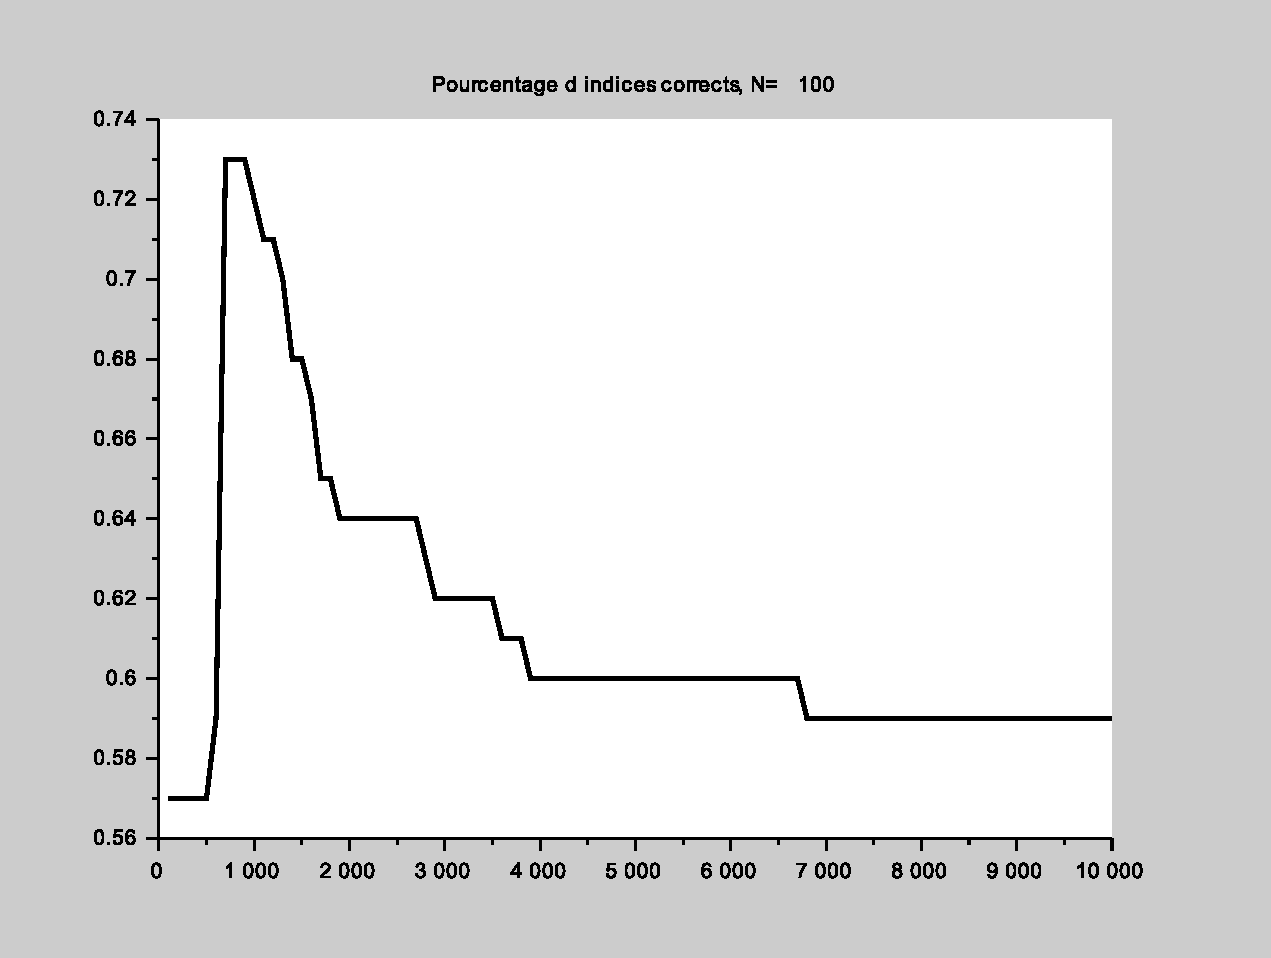
\includegraphics[scale=0.3]{percent_alpha2_100.pdf}
\caption{Pourcentage d'indices valides pour $N=100$}
\end{minipage}
\begin{minipage}[b]{.46\linewidth}
\centering
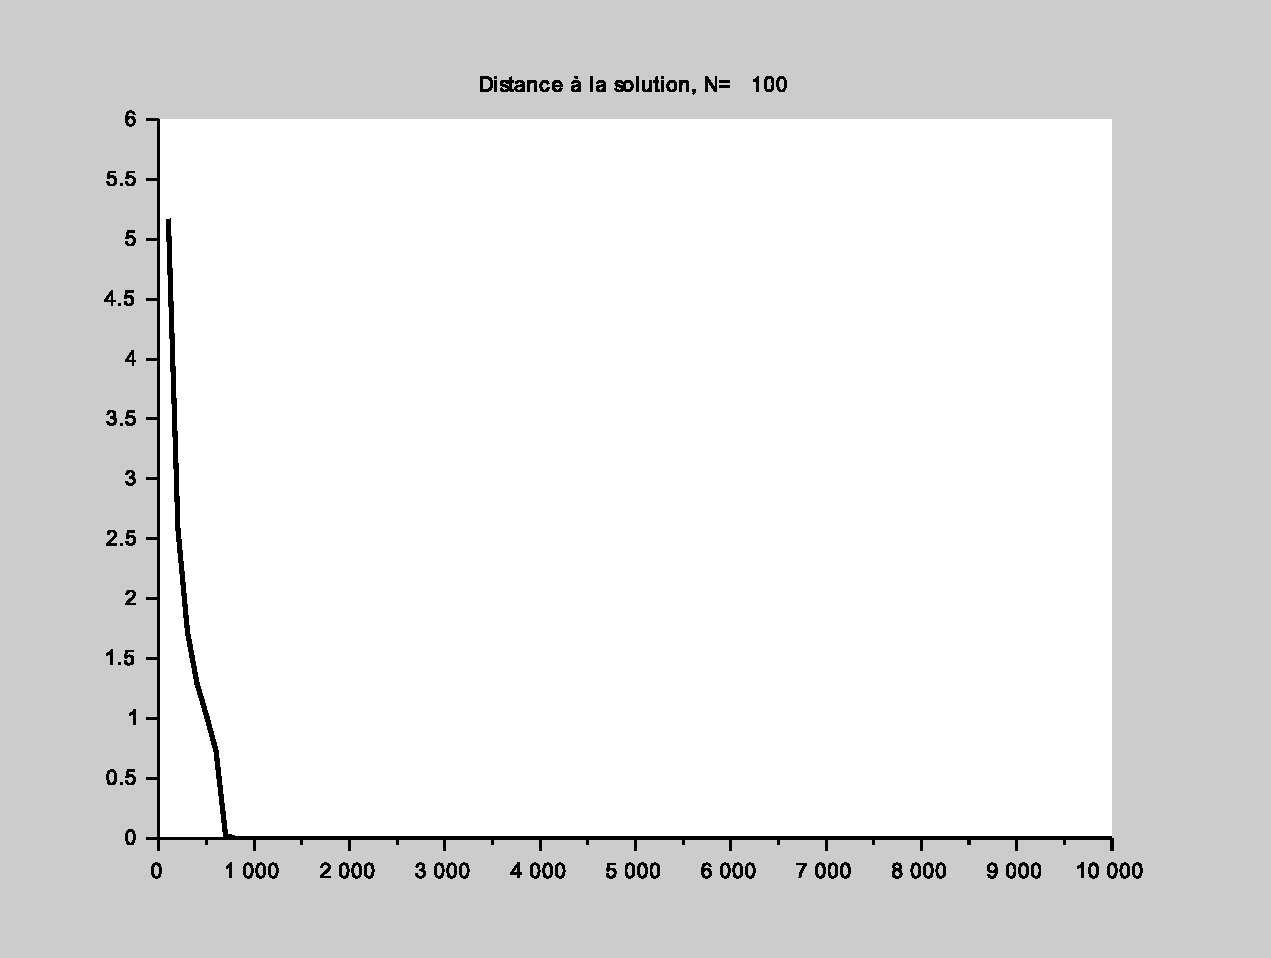
\includegraphics[scale=0.3]{dist_alpha2_100.pdf}
\caption{Distance entre la dernière itération et l'avant-dernière pour $N=100$}
\end{minipage}
\end{figure}
Ici on étudie l'évolution du nombres d'indices corrects, c'est-à-dire tels que $(Ax)_i \le b_i$.
On constate que les résultats se situent d'abord autour d'une moitié d'indices corrects ce qui n'est pas satisfaisant.
On constate que pour ces $\alpha$ trop faibles l'algorithme n'a pas convergé.
Ensuite, on observe une forte augmentation puis une décroissance stricte du nombre d'indices corrects.
Cela est dû au fait qu'on cherche de plus en plus à minimiser la norme de $x$ sans chercher à minimiser la norme de $(Ax-b)_+$.
Conformément à ce qu'on attendait, il s'agit de prendre $\alpha$ le plus petit possible pour que le plus d'inégalité soient satisfaites.
\begin{figure}[H]
\centering
\begin{minipage}[b]{.46\linewidth}
\centering
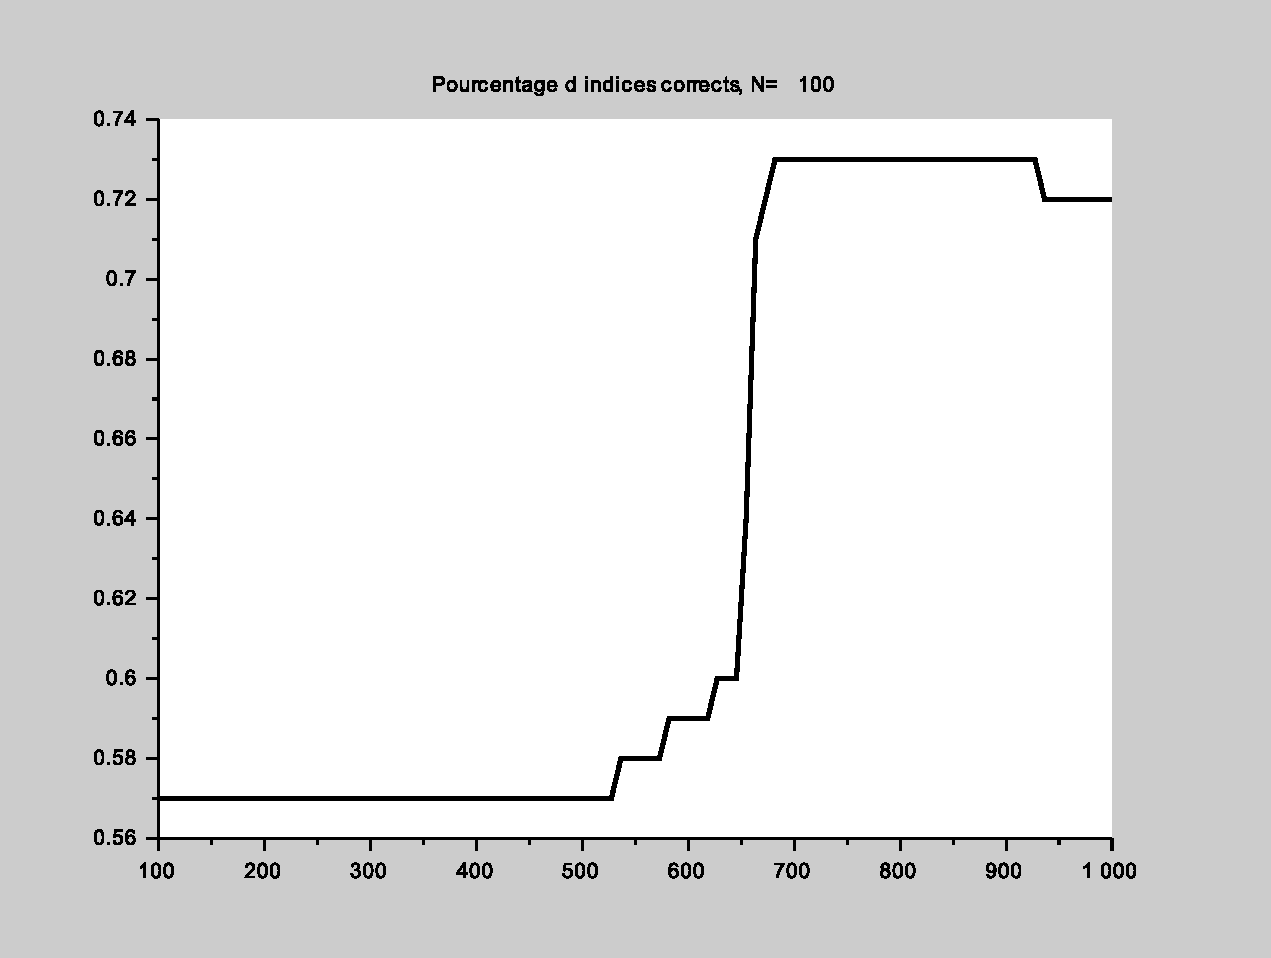
\includegraphics[scale=0.3]{percent_alpha1_100.pdf}
\caption{Pourcentage d'indices valides pour $N=100$}
\end{minipage}
\begin{minipage}[b]{.46\linewidth}
\centering
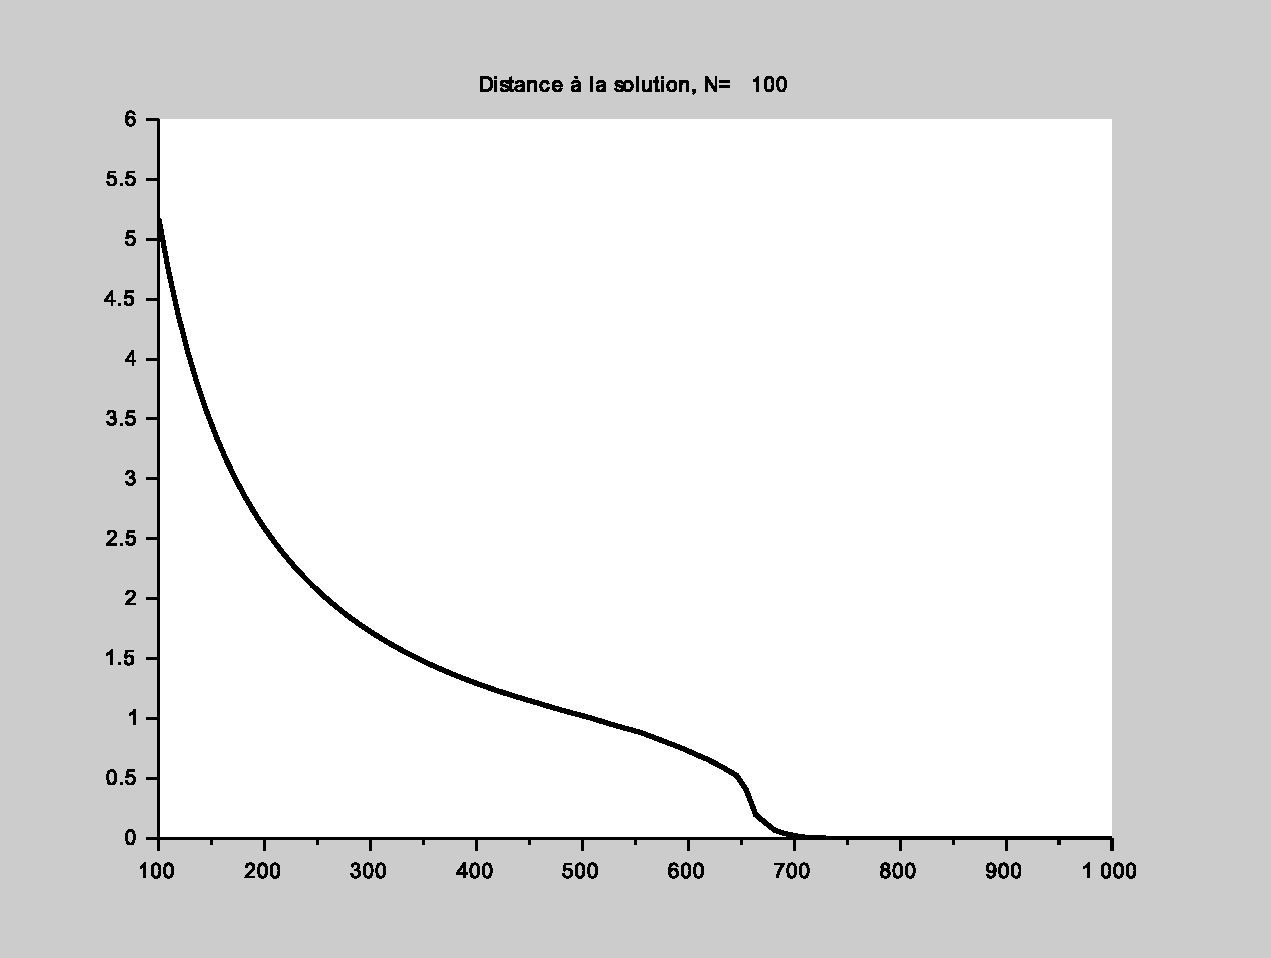
\includegraphics[scale=0.3]{dist_alpha1_100.pdf}
\caption{Distance entre la dernière itération et l'avant-dernière pour $N=100$}
\end{minipage}
\end{figure}
Ici, on a détaillé le comportement de l'algorithme lorsque $\alpha$ est petit.
Il est clair que l'augmentation du nombre d'indices corrects est dû à la convergence de l'algorithme.
Néanmoins, au maximum, seuls $74$ indices sur $100$ vérifient les contraintes.
Pour faire mieux il serait souhaitable de diminuer la valeur de $\alpha$.
Malheureusement on perd alors la convergence.
\begin{figure}[H]
\centering
\begin{minipage}[b]{.46\linewidth}
\centering
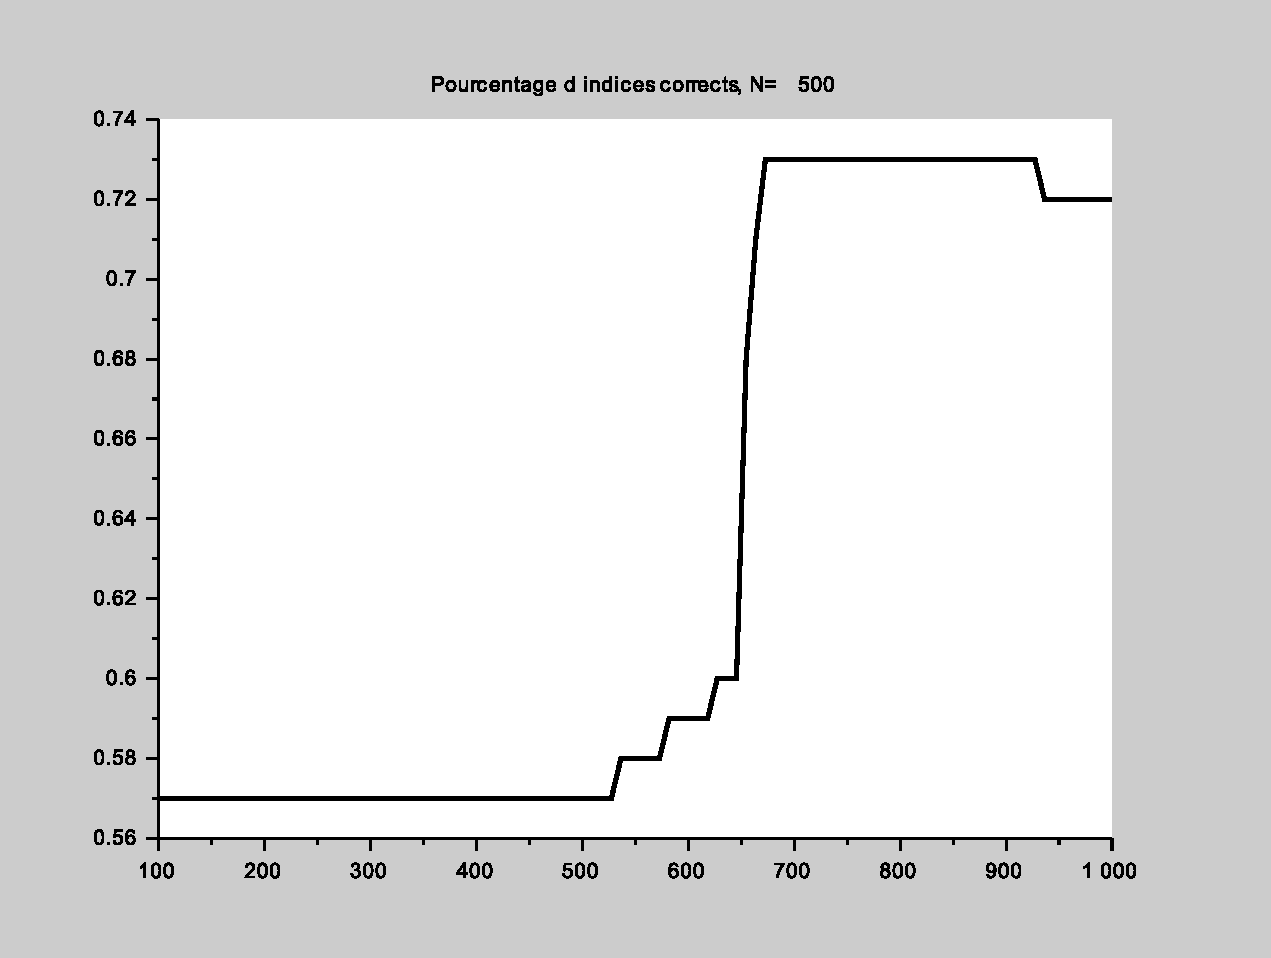
\includegraphics[scale=0.3]{percent_alpha1_500.pdf}
\caption{Pourcentage d'indices valides pour $N=500$}
\end{minipage}
\begin{minipage}[b]{.46\linewidth}
\centering
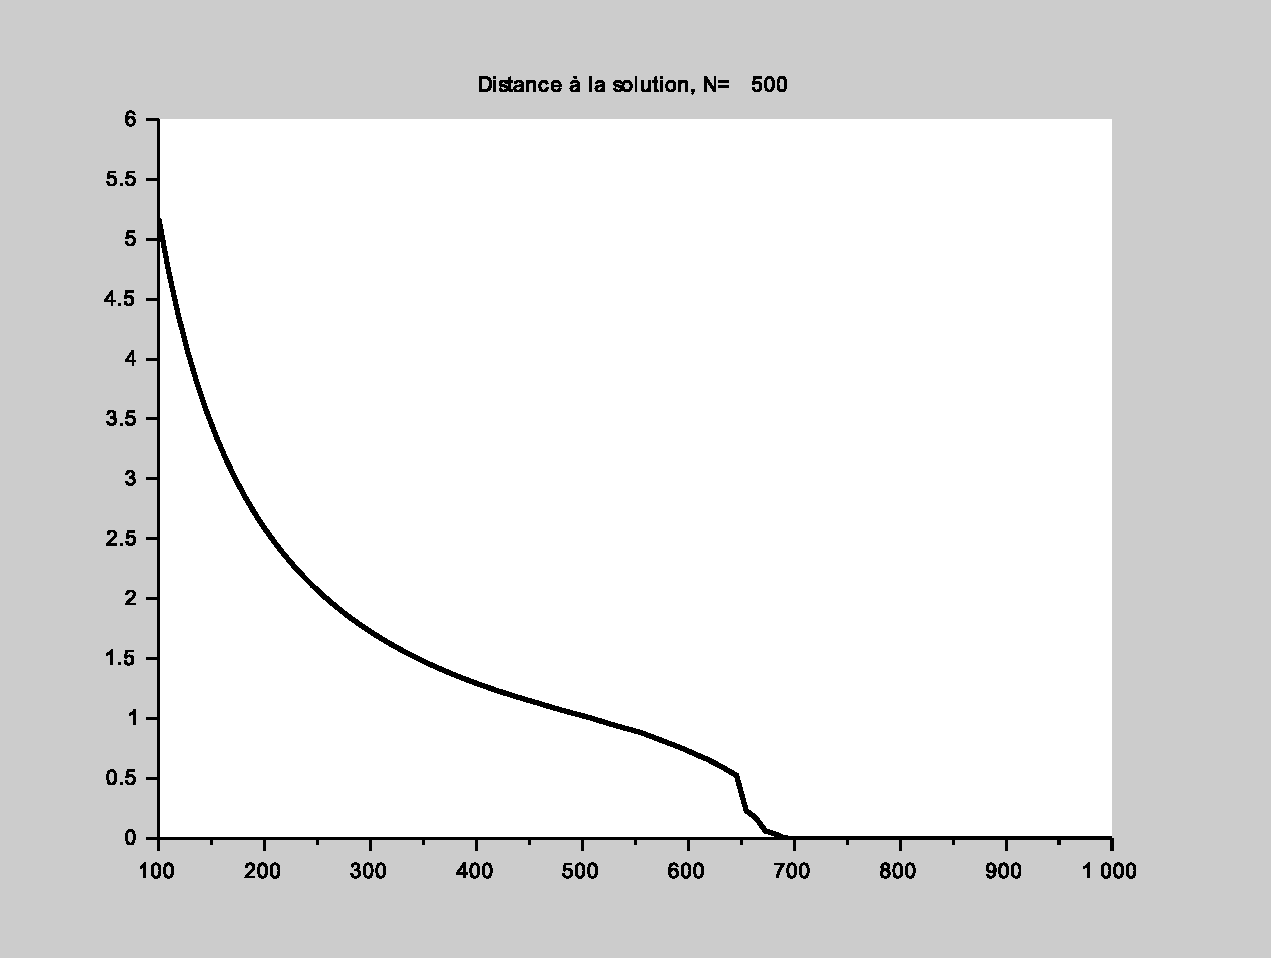
\includegraphics[scale=0.3]{dist_alpha1_500.pdf}
\caption{Distance entre la dernière itération et l'avant-dernière pour $N=500$}
\end{minipage}
\end{figure}
On a ici tenté d'augmenter le nombre d'itérations de l'algorithme afin de déterminer si le problème de la non-convergence est dû à un $\alpha$ trop petit ou à un nombre d'itérations trop faible.
Le fait que les résultats soient quasiment lorsque $N=500$ nous incite à pencher vers la première hypothèse d'un $\alpha$ trop petit.

\section{Une autre approche du problème}

\subsection{Du cas d'inégalité au cas d'égalité sous contrainte}
\begin{thm}
  Soient $A \in \mathcal{M}_{n,m}(\mathbb{R})$ avec $(n,m) \in \mathbb{N}^2$ et $b \in \mathbb{R}^{n}$.
  Il existe $(n', m') \in \mathbb{N}^2$ et $A' \in \mathcal{M}_{n',m'}(\mathbb{R})$ et $b' \in \mathbb{R}^{n'}$ tels que le système d'inégalité linéraire
\begin{align*}
  Ax &\leq b\\
\end{align*}
soit équivalent au sytème d'égalité lineaire avec contrainte:
\begin{align*}
  A'x &= b'\\
  x &\geq 0\\
\end{align*}
\end{thm}

\subparagraph{Remarques :}
\begin{itemize}
  \item TODO
\end{itemize}

\subparagraph{Démonstration :}
On pose $z = Ax -b$ de sorte que le système $Ax \leq b$ est équivalent à:
\begin{align*}
  z &\geq 0 \\
  Ax + z &= b
\end{align*}
On pose $x_+ = max(x, 0)$ et $x_- = max(-x, 0)$ de sorte que:
\begin{align*}
  x_+ &\geq 0 \\
  x_+ &\geq 0 \\
  \tilde{A} &= \left[ A, -A, Id \right]\\
  \tilde{x} &= \left[ \begin{array}{c} x_+ \\ x_- \\ z \end{array} \right]\\
\end{align*}
et on a bien :
\begin{align*}
  \tilde{A}\tilde{x} &= Ax + z = b\\
  \tilde{x} \geq 0
\end{align*}
qui est équivalent au système $Ax \leq b$.

\subsection{Algorithme de gradient projeté}

Ce problème d'égalité sous contrainte que nous avons énoncé peut être résolu au sens des moindres carrés.
Les conditions d'optimalité KKT donnent:
\begin{align*}
  \tilde{A}^T \left( \tilde{A}\tilde{x} - b \right) &= \Lambda\\
  \Lambda \geq 0\\
\end{align*}

\bibliographystyle{plain}
\bibliography{report_project}

\end{document}
